\section{Background and Motivation}
\subsection{Distributed Transactions}
Transactions are a widely used programming abstraction in shared data programming.
Data operations enclosed by transactional begin() and end() calls, are guaranteed to be
executed atomically. Furthermore, transactional runtimes guarantee isolation and consistency
properties for the executed transactions and in the case of database like runtimes, they also
provide durability for the executed transactions.

However, the current application data sets are large enough -- they often do not fit in to
single database runtime with local storage stack are thus the data is partitioned across the
multiple storage runtimes. Such paritioned data stores can be programmed by same transactional 
abstraction and protocols involved in such setting is known as distributed transactions.
Distributed transactions and related protocols have been extensively studied over the years in the
database community.
\subsection{Motivation for system redesign}
Recent hardware and application trends motivate us to rethink the mechanisms involved in
distributed transactions.
\begin{itemize}

	\item{\bf NVM}
		Non-volatile memory technologies such as 3DXpoint by intel promises memory speed persistent
		writes. The form factor of these new memories are smaller than that of DRAM main memory -- these 
		new memory devices are ideal as main storage hardware. However, the NVMs provide applications with
		memory bus based load/store interface, thus existing DB storage stacks my not yield the optimal performance.
	\item{\bf RDMA} Provides high bandwidth network communication between compute nodes. RDMA enabled NICs are

		capable of directly writing to the target application's userspace memory. Thus RDMA enables remote
		CPU bypass with one-sided read/write primitives and also supports atomic remote fetch\_and\_add instructions.
		While there has been work on efficient RDMA based RPC implementations, exploiting best perforance out of 
		RDMA one-sided primitives often requires application data storage layout re-structuring.
	\item{\bf KV-stores}
		Conventional database schemes were based on relational data model and had strict contrains on database schemas.
		Recent enterprise applications have opted for more relaxed storage layouts in the form of key-value stores.
		In its simplest form key-value stores are similar to hash-table structure supporting put/get operation semantics.
		When designing distributed transactions for kv-stores, we may able to better optimize protocol stepts for the 
		simple storage layout of the backing store.

\end{itemize}

The above trends in the storage, network and applications allow us to rethink the distributed 
transactions protocols. Specifically, we hypothize that transactions that are based on optimistic
concurrency control mechanisms have more opportunity to exploit the low latency, high bandwidth
network/storage stacks. However, naive integration of these components not going to yield the 
best overall system performance as conventional bottlenecks tend to move with changes in 
technology parameters. Next, we are going to look at the specifics on OCC protocol we are going to 
look at.


\subsection{Snapshot isolation based distributed transactions}

\begin{figure}[]   
	\centering
	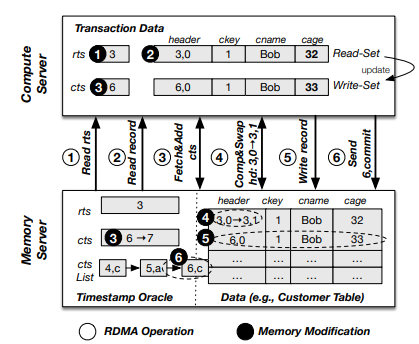
\includegraphics[width=\linewidth]{figures/SI.png} 
	\caption{\small Naive RDMA based SI protocol. The diagram is from the NAM-DB paper. I did not try to invent things again.} 
	\label{fig:si} 
\end{figure}

We now look at a distributed transactional steps happening in a 
multi-versioned key-value store that uses optimistic concurrency control (OCC)
as the concurrency control mechanism. The transactions operate under data consistency
model named snapshot isolation. We briefly introduce them here as we use the terms 
extensively in the text to follow.

\noindent{\bf multi-versioning}
We create a new copy of the data for each update and associate with a version. Furthermore, we record the 
begin and end timestamps of the trsansction ids that created/updated the data. The key idea here is that
incoming transactions figure out the visibility of data based on these timestamps. As a rule of thumb, you
can read data from future.

\noindent{\bf OCC}
We copy/read the data in a private workspace during transactional execution. The writes get updated in the 
local copy as well. The speculative workspace update get merged in to master data versions at the very
end of the transaction -- we call this transaction commit. Conflicting writes results in transaction aborts.

\noindent{\bf snapshot-isolation}
Defines the transactional data consistency model. Each transaction works on a snapshot of the database that
existed at the begin of the transaction. The snapshot is logically constructed using begin, end timestamps of the
versioned data. Snapshot isolated transactions are not serializable.

Executing transaction involves first fetching the read timestamp (rts). rts value defines the logical database
snapshot for the transaction. Subsequent reads for a specific key is fetched from the multiversioned data table
based on the visibility rules using RDMA reads (step 1 in ~\ref{fig:si}) in to the local sandboxed memory.(e.g the tuple with ckey\=3 in
the example). The writes are buffered in the sandboxed memory as well. 

During the commit step, the transaction execution thread fetches a unique commit timestamp (cts)
from the memory server/global counter ( step 3 in Fig ~\ref{fig:si}). At the commit time, 
transaction exuecution thread/compute server verifies and locks all records in its write-set on
the memory servers by locking each of the key entreis. The key idea is to check if the write-set
entries has been modified since their last read -- which signals possible conflict. After the verification
step the speculative updates get merged in to the versioned data store -- while holding the latches
for each of the write-set keys.

The above discussion on snapshot-isolated MVCC transactions is aimed at giving the bare minimal
knowledge to understand rest of the paper. For thorough discussion on the topic we recommend~\cite{namdb}.

\subsection{The Need for scalable timestamps}

The previously described global timestamping mechanism is not scalable~\cite{rethinking}, both
in node local multi-core and distributed environment.
First, for each remote transaction, execution thread has to do a RDMA atomic fetch-and-add 
operation to a same memory location ( unique per partition ) to create a unique timestamp.
Atomic RDMA operations requires latching in the NIC hardware level and scales poorly with the
concurrent accesses -- number of transaction execution threads.
Scalability of RDMA atomic instructions based timestamps is not limited to above~\cite{namdb}.


Next, fat compute nodes with hundreads of CPU cores and terabytes DRAM/NVM memory is going
to be a norm in enterprise computing. Smart data partitioning schemes on the dataset aim to
eliminate distributed transactions by converting them in to node local transactions.
However, transactional operational involving local data updates still needs to be ordered 
to maintain correct concurrency and data consistency duarantees. The conventional atomic
counters based timestamping scales poorly across cores and NUMA sockets~\cite{ordo}. This 
is because atomic instructions involves costly cache-coherence transactions to avoid 
concurrent modifications to the data.


We argue that it is important to design a scalable timestamping mechanism that is 
optimized for both node local transactions and remote transactions as it is the most 
heavily used deployment model found in enterprise.
Related work such as, NAM-DB~\cite{namdb} does not have a notion of local
data updates, as the compute is always remote to the data. On the other spectrum, 
systems like ~\cite{cicada} only solves scalability in node local transactions.
In this work, we propose scalable timestamps technique that is optimized for both
node local and remote transactions.



\begin{figure}[]   
	\centering
	\includegraphics[width=\linewidth]{figures/gtecho.pdf} 
	\caption{\small } 
	\label{fig:gtecho} 
\end{figure}
